\chapter{The influence of the group environment}\label{chap:env}

\section{Introduction}\label{sec:intro}
 
 So far, I have considered mergers, interactions, morphology and AGN as causes of quenching across the galaxy population. While it is clear that these mechanisms can strongly affect the SFHs of galaxies, the density of a galaxy's environment is thought to be the largest influence on the evolutionary path the galaxy can take. 
 
 The galaxy environment as a cause of quenching was proposed due to the correlation of morphology \citep{dressler80, smail97, poggianti99, postman05, Bamford09}, star formation rate (SFR) and the quenched galaxy fraction \citep{kauffmann03, Baldry06, peng12, darvish16} with environmental density. Star forming disc galaxies tend to be located in low-density environments with quiescent elliptical galaxies in more dense environments. Although these correlations were originally interpreted as causation, recent evidence from simulations suggests that the environment may not be the dominant quenching mechanism in the galaxy lifecycle \citep{ref, ref} with \citet{skibba09} suggesting that the morphology-density relation is mostly due to the colour-density relation as seen in \citet{pimbblet02}. Perhaps instead, the correlation of increased galaxy quenched fractions with environment is due to a superposition of the effects of mergers \& interactions and both mass \& morphology quenching. 
  
In order to isolate the cause of the density-morphology and density-SFR correlations, I need to observe how morphology and galaxy quenching timescales change in group environments with different properties in comparison to the field. Here, I use the group environment to tackle this problem, as this is a more typical environment for a galaxy than the relatively rare rich cluster environment \citep{carlberg04}. I construct a sample of both group and field galaxies and once again use \starpy\ to determine the quenching time and rate to describe a simple SFH for a galaxy given its photometry. However, dense environments are messy with many factors at work, whose effects are difficult to discern. These individual mechanisms effects would be washed out across the population density distributions produced by \textsc{popstarpy} and so I do not employ this method in this Chapter. 

Instead, I have simplified the analysis in order to separate the effects of the different quenching mechanisms contributing to the galaxy population in the group environment. I aim to determine the following: (i) How does the environment influence the detailed morphological structures of a galaxy?  (ii) Is quenching which is directly caused by the environment occurring in galaxy groups?

%In Section~\ref{sec:data} I describe the group catalog employed and highlight the results in Section~\ref{sec:results}. 
 
\section{Data and Methods}\label{sec:data}

\subsection{Group Identification}\label{sec:groups}

The selection of a robust cluster or group catalog is a thesis in itself, with many studies attempting this across the SDSS \citep{} and other large surveys \citep{}. Difficulties arise in removing projection effects, understanding the selection function used, covering large ranges in mass and redshift, and dealing with spectral fibre collisions \citep[see comprehensive review by][for in depth discussion]{postman02}. Various different methods have been employed to achieve robust group identification including clustering algorithms \citep[e.g.][]{nichol01, miller05}, galaxy colour modelling \citep{annis04}, adaptive filter halo modelling \citep{yang05, yang07} and friends-of-friends algorithms \citep{goto05, merchan05, berlind06}. 

Each group finding algorithm has to be tested for purity (how contaminated the groups are by non-members) and completeness (how often are true members excluded from a group). \citet{campbell15} compared the purity and completeness of two of the most frequently used group catalogs of \citet[][a friends-of-friends algorithm]{berlind06} and \citet[][a halo modelling algorithm]{yang07} and concluded that no sample could achieve perfect purity or completeness. Despite the different algorithms employed to identify group galaxies in the two catalogs, \citeauthor{campbell} found that the two catalogs are remarkably similar; however the \citeauthor{yang07} catalog has higher purity of satellites at lower halo masses (i.e. the low halo mass groups are less contaminated by non-members). For this reason the \citeauthor{yang07} is the most commonly used catalog across environment studies using the SDSS \citep{citationbomb}, however I find that when cross matched with the \textsc{gz2-galex} sample (with a $3``$ search radius) only $38$ galaxies (of $176,604$ galaxies with more than 2 galaxies in a group) are identified. This is most likely due to the necessity for GALEX NUV photometry. 

Instead I therefore use the \citet{berlind06} catalogue, which uses a friends-of-friends algorithm to identify group and cluster galaxies in the SDSS. This was cross matched to the \textsc{gz2-galex} sample and limited to $z < 0.1$ (to ensure GALEX completeness of the red sequence; see \citealt{wyder07, yesuf14}) to give $14,199$ group galaxies. Centrals were selected as the most massive galaxy in a group \citep[as in][]{yang07, yang09, pasquali10} with all other galaxies in a group designated as satellites and the number of galaxies in a galaxy's group, $N_{group}$ was recorded. 

The projected group centric radius, $R$, of all satellite galaxies was calculated from the projected separations of the co-ordinates of a satellite from its central; this was then converted to $\rm{kpc}$ from a consideration of the observed redshift of the central galaxy. In order to compare groups of different sizes, the virial radius is often used as a normalisation constant to this projected group centric radius. Here I use a proxy to the virial radius \citep[see][]{navarro95}, $R_{200}$, the radius within which the group mass overdensity is 200 times the critical density, $\rho_{\rm{crit}}(z)$, as defined by \citealt{finn05}:
\begin{equation}\label{eq:overdense}
200\rho_{\rm{crit}}(z) = \frac{M_{cl}}{\frac{4}{3}\pi R_{200}^3}
\end{equation}

where $M_{cl}$ is the mass of the group. \citeauthor{finn05} then use the $z$ dependance of the critical density and the virial mass to relate the line-of-sight velocity, $\sigma_x$, to the group mass so that $R_{200}$ becomes:
\begin{equation}\label{eq:r200}
R_{200} = 1.73 \left ( \frac{\sigma_x}{1000 \rm{km}~\rm{s}^{-1}} \right) \cdot \frac{1}{\sqrt{\Omega_{\Lambda} +\Omega_o(1+z)^3}} ~ h_{100}^{-1} ~\rm{Mpc}, 
\end{equation}

where $\sigma_x$ is the line-of-sight velocity dispersion of a group. This was calculated from the proper velocities of each galaxy, $i$ as defined in \cite{danese80}:
\begin{equation}\label{eq:propervel}
v_i = c \cdot \frac{z_i - z_{group}}{1 + z_{group}}.
\end{equation}
The line-of-sight velocity dispersion, $\sigma_x$, was then calculated for a group as the standard deviation of the velocity dispersions $\sqrt{(v_i - \left< v_i\right>)^2}$. These calculations resulted in a sample of $3,468$ centrals and $10,731$ satellites within a projected group centric radius range of $0 < R/R_{200} < 25$ and $z < 0.084$ which shall be referred to as the \textsc{gz2-berlind} sample. Note that for a galaxy (central or satellite) to be included in the \textsc{gz2-berlind} sample, the rest of its group does not, however the properties of that group are still retained by the included galaxy. 

Unlike in previous Chapters, here I will specifically focus on galaxies that are below the star forming sequence (SFS). I therefore select galaxies that are $1\sigma$ below the SFS, giving $4,629$ satellite and $2,314$ central galaxies which will collectively be referred to as the \textsc{gz2-group} sample. These galaxies are shown in the panels of Figure \ref{fig:sfrmass} and can be seen to lie below the SFS of star formation. 

\begin{figure}
\centering
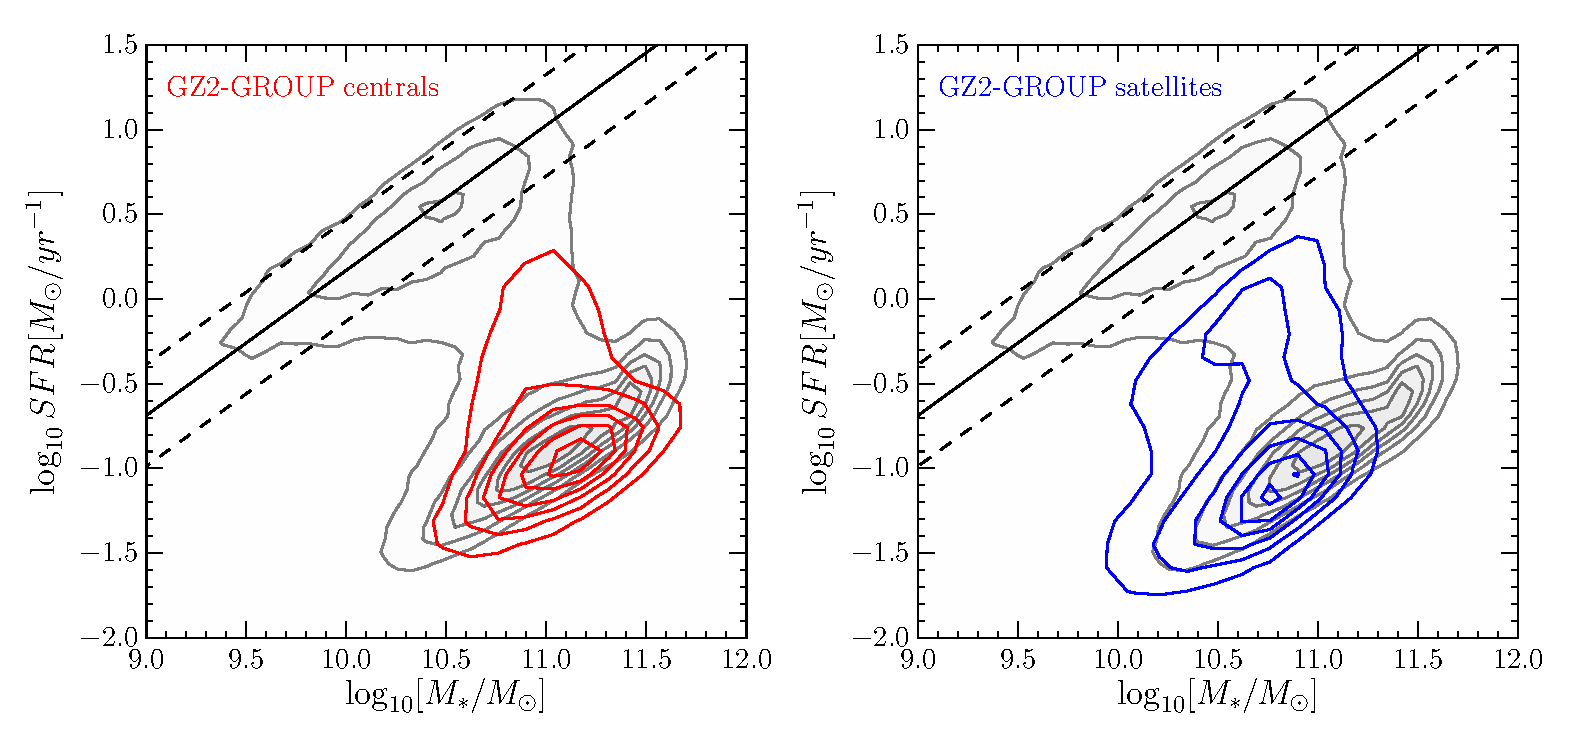
\includegraphics[width=\textwidth]{environment/sfr_mass_quenched_centrals_satellites_gz2_group.pdf}
\caption[Stellar mass-SFR plane for the centrals and satellites of the \textsc{z2-group} sample]{The stellar mass-SFR plane showing central (left; red contours) and satellite (right; blue contours) in the \textsc{z2-group} sample. In both panels the entire SDSS sample from the MPA-JHU catalog is shown by the grey contours. The definition of the SFMS from \cite{peng10} at $\overline{z} = 0.053$ (solid line, the mean redshift of the \textsc{gz2-group} sample) with $\pm1\sigma$ (dashed lines) is shown.}
%KS Test between distributions?
\label{fig:sfrmass}
\end{figure}


I also compare the \textsc{gz2-berlind} and \textsc{gz2-group} samples with a measurement of the projected neighbour density, $\Sigma_N = N/4\pi d_N^2$, from \cite{Baldry06} where $d_N$ is the distance to the $N^{\rm{th}}$ nearest neighbour. In this work I use the estimates of \cite{bamford09} of a local galaxy density, $\Sigma$, determined by averaging $\log\Sigma_N$ for $N = 4$ and $N=5$. $90\%$ of the \textsc{gz2-berlind} sample have $\log\Sigma > -0.8$ (the threshold quoted by \citealt{Baldry06} below which field galaxies are found), suggesting high completeness of the sample. The distributions of $\log\Sigma$ for star forming and quenching/quenched centrals and satellites in the \textsc{gz2-berlind} sample are shown in Figure~\ref{fig:sigmadist}. Star forming galaxies tend to reside in less dense local environments than their quenching/quenched counterparts. The satellite galaxies as a whole also seem to occupy denser local environments than centrals, however on investigation this seems to arise because the satellites in the \textsc{gz2-berlind} sample reside in groups with larger $N_{group}$ than the centrals. This is once again likely due to the necessity for GALEX colours. 

\begin{figure}
\centering
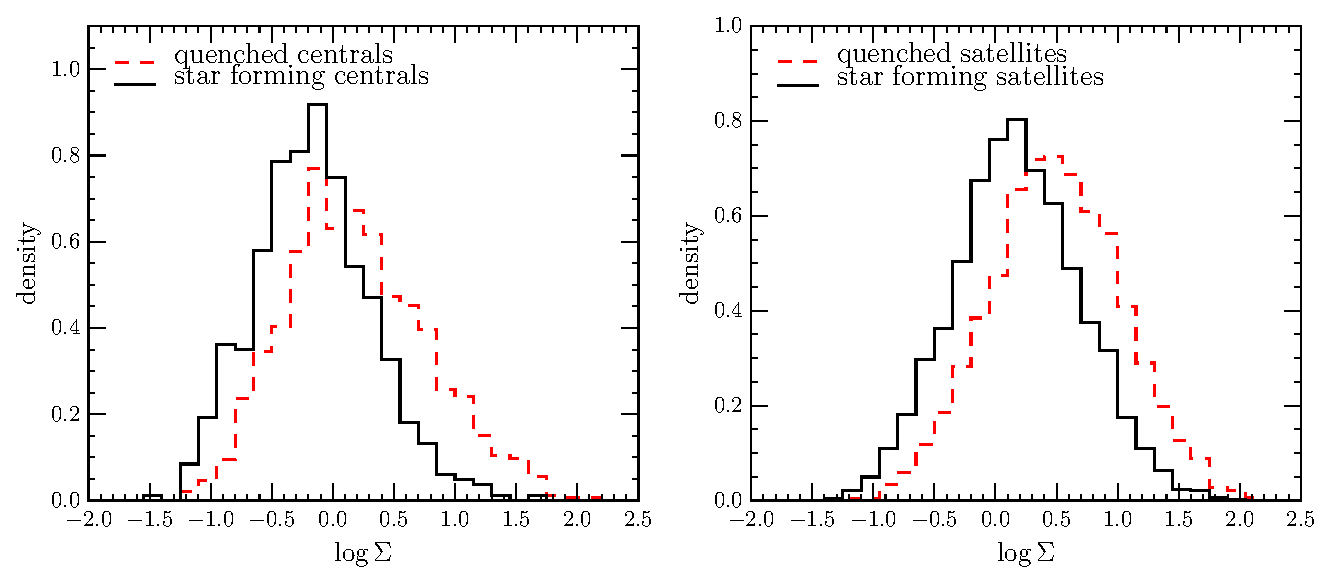
\includegraphics[width=\textwidth]{environment/SIGMA_density_sf_q_cent_sat.pdf}
\caption[Local environment density distributions of central and satellite galaxies]{Local environment density, $\log\Sigma$, distributions of star forming (black) and quenching/quenched (red) central (left) and satellite (right) galaxies in the \textsc{gz2-group} sample.}
%KS Test between distributions?
\label{fig:sigmadist}
\end{figure}


\subsection{Field sample}\label{sec:field}

For all galaxies in the \textsc{gz2-galex} sample, I calculated the smallest projected group centric radii, $R/R_{200}$, from each of the central galaxies in the \citet{berlind06} catalog (regardless of whether a central was included in the \textsc{gz2-berlind} sample) and selected candidate field galaxies as those with (i) $R/R_{200} > 25$ and (ii) $\log\Sigma < -0.8$ \citep[the threshold on the local environment density which selects field galaxies as defined by][]{Baldry06}. I chose to use both of these environmental density measures ensure a pure sample of candidate field galaxies.

This sample of field galaxy candidates was then matched in redshift and stellar mass firstly to the central galaxies of the \textsc{gz2-group} sample to give $2,309$ field galaxies with $z < 0.084$ which will be referred to as the \textsc{gz2-cent-field} sample. In this work I shall focus on galaxies which are either quenching or quenched and are more than $1\sigma$ below the SFS. This encompasses $1,596$ field galaxies with $z < 0.084$ which will be referred to as the \textsc{gz2-cent-field-q} sample. It will be used as a control sample when investigating the trends with central galaxy properties of the inferred quenching parameters. The redshift distribution of the \textsc{gz2-cent-field-q} sample is shown in comparison to the distribution of central galaxies in the \textsc{gz2-group} sample in left panel of Figure~\ref{fig:zcompare}. %SDSS images of a random selection of galaxies from the \textsc{gz2-group} and \textsc{gz2-cent-field-q} samples are shown ordered by their GZ2 debiased vote fraction in Figure~\ref{fig:mosaic}. %KS test between samples?

Secondly, the field galaxy candidates were then matched in redshift and stellar mass to the satellite galaxies of the \textsc{gz2-group} sample to give $5, 004$ field galaxies with $z < 0.084$ which will be referred to as the \textsc{gz2-sat-field} sample. These galaxies in the \textsc{gz2-sat-field} sample will be used as a control when investigating the morphological trends of satellite galaxies with environment. Note that the sample is not restricted to being $1\sigma$ below the SFS in this case. The redshift distribution of the \textsc{gz2-sat-field} sample is shown in comparison to the distribution of satellite galaxies in the \textsc{gz-group} sample in the right panel of Figure~\ref{fig:zcompare}

We obtain SFRs and stellar velocity dispersions of galaxies for all of the field samples described above from the MPA-JHU catalogue \citep{kauffmann03, brinchmann04}. 

\begin{figure}
\centering{
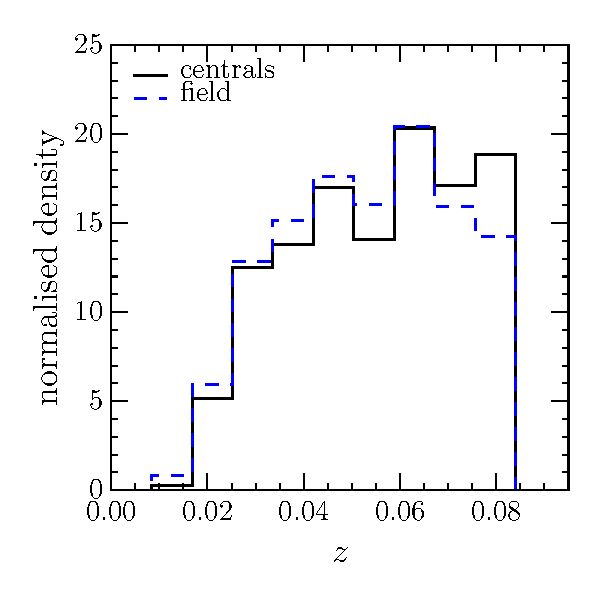
\includegraphics[width=0.45\textwidth]{environment/redshift_cent_field.pdf}
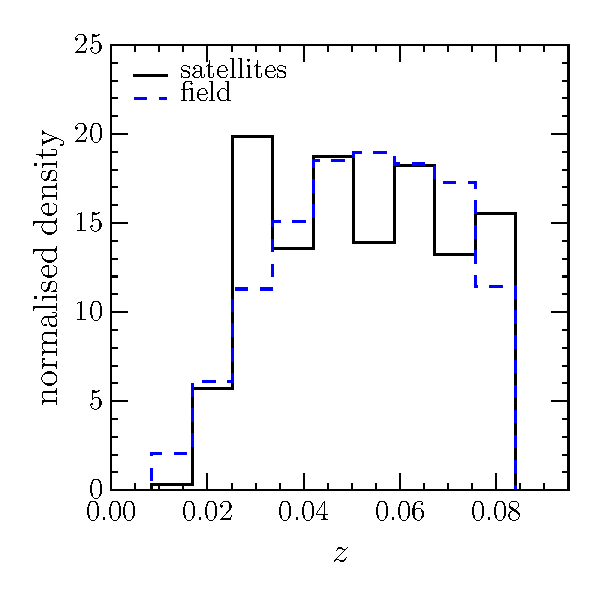
\includegraphics[width=0.45\textwidth]{environment/redshift_sat_field.pdf}}
\caption{Redshift distributions of central (left) and satellite galaxies (right) in the \textsc{gz2-group} sample (black solid line) in comparison the redshift matched \textsc{gz2-cent-field-q} (left; blue dashed line) and \textsc{gz2-sat-field} samples (right; blue dashed line).}
%KS Test between distributions?
\label{fig:zcompare}
\end{figure}

\subsection{Morphological fractions}\label{sec:morphfrac}

I once again utilise the GZ2 vote fraction to quantity the morphology of galaxies in the \textsc{gz2-group} sample, in order to investigate the morphological trends with group radius. As in previous Chapters, I shall utilise $p_{\rm{disc}}$ and $p_{\rm{smooth}}$ but will also use $p_{\rm{bar}}$, $p_{\rm{bulge}}$ and $p_{\rm{merger}}$ to calculate the bar, bulge and merger fractions in the \textsc{gz2-group} sample respectively. 

Fractions are calculated considering the number of barred ($p_{\rm{bar}} > 0.5$; see \citealt{masters11a, cheung13}) and bulged ($p_{\rm{bulge}} > 0.5$) galaxies over the number of disc galaxies ($p_{\rm{disc}} > 0.43$, $p_{\rm{edge\_on, no}} > 0.715$, $N_{\rm{edge\_on, no}} > 20$; see Table~\ref{table:gz2thresholds}, originally printed in \citealt{GZ2}) in the \textsc{gz2-group} satellite sample. The merger fraction considers the number of merging galaxies ($p_{\rm{merger}} > 0.4$; see \citealt{darg10a}) over the number of galaxies in the \textsc{gz2-group} satellite sample. 

\subsection{Time since quenching}\label{sec:delta}

The SFHs of all galaxies in both the \textsc{gz2-group} and \textsc{gz2-field} samples were analysed using \starpy\; the output of \starpy\ is probabilistic in nature, providing the posterior probability distribution across the two-parameter space for an individual galaxy. Whereas in Chapters~\ref{chap:morph} \& \ref{chap:agn} the \textsc{popstarpy} method was used to combine and weight the individual distributions to give an overall distribution representing the population of galaxies, due to the complex nature of the group environment, in this Chapter I instead take the 50th percentile walker position of an individual posterior probability distribution to give the most likely $t_{q}$ and $\tau$ for each galaxy. \

This simplifies the output from \starpy  ~for each galaxy from a probability distribution to just values, with uncertainties which encode the information about the shape of the individual galaxy's SFH posterior probability distribution. In this Chapter I will look for trends in the time since quenching onset, $\Delta t$, for a given galaxy by calculating {\bf $\Delta t = t_\mathrm{obs} - t_{q}$}. I will observe how this quantity changes with group properties, including the halo mass, velocity dispersion, number of group members and relative velocity of a satellite galaxy. 


\section{Results}\label{sec:results}

\subsection{Mass dependance with radius}

Since morphological features have been shown to be dependent on the stellar mass of a galaxy \citep[e.g. the increase in the bar fraction with stellar mass][]{skibba12}, before investigating trends in the morphology with group radius in the \textsc{gz2-group} sample, the mass dependence on the group radius must be considered. This is shown in Figure~\ref{fig:massdep}. The average mass is roughly flat and consistent with the median field value with increasing group radius, until the most central group radius bin at $R \sim 0.01~R_{200}$. This trend is present for both morphologies, with early-type galaxies showing a larger increase in the average stellar mass. This trend with stellar mass should be kept in mind as a potential bias to the results presented in the following sections. 

\begin{figure}
\centering{
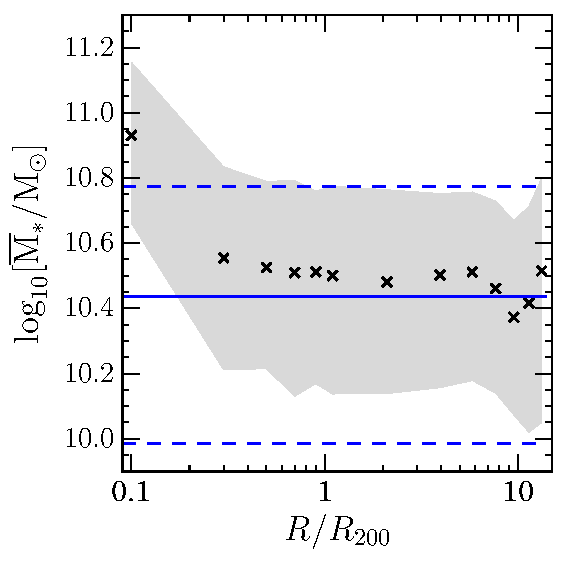
\includegraphics[width=0.45\textwidth]{environment/mass_trend_with_log_radius_compare_field.pdf}}
\caption[Average mass with group radius in the GZ2-GROUP sample]{The average stellar mass as a function of radius from the group centre. The shaded regions show the $\pm1\sigma$ in each bin of $R/R_{200}$. The average stellar mass of the \textsc{gz2-sat-field} sample is also shown (blue solid line) with $\pm1\sigma$ (blue dashed line).}
\label{fig:massdep}
\end{figure}

\subsection{Dependence of detailed morphological structure with environment}

\begin{figure}
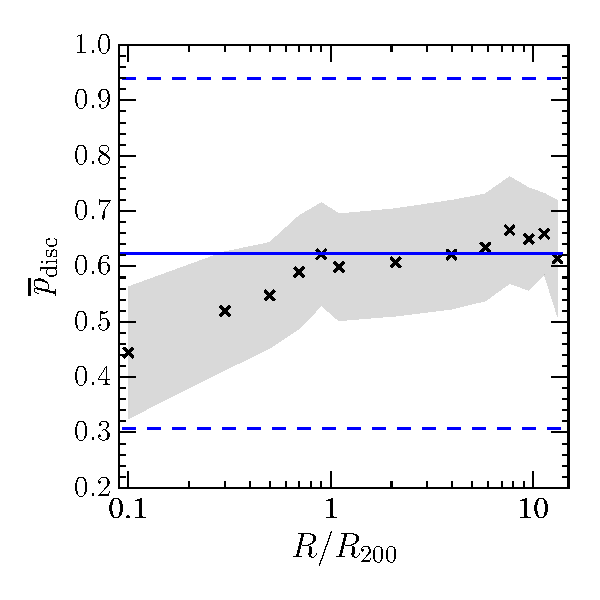
\includegraphics[width=0.46\textwidth]{environment/p_disc_trend_with_log_radius_field_compare.pdf}
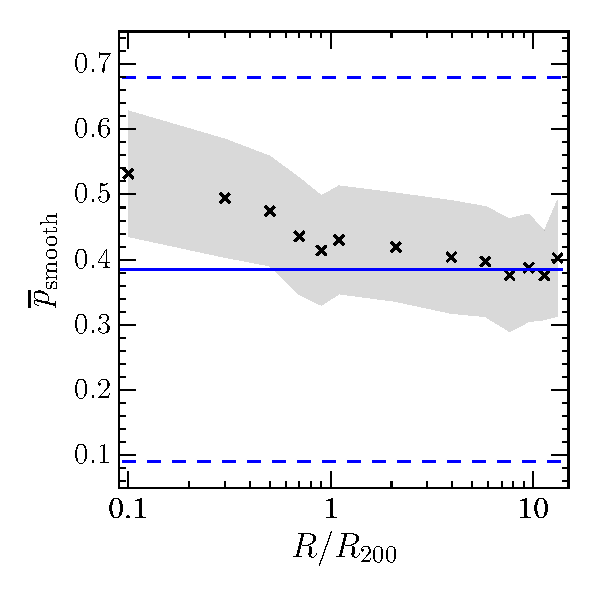
\includegraphics[width=0.46\textwidth]{environment/p_smooth_trend_with_log_radius_field_compare.pdf}
\caption{Mean GZ vote fraction for disc (top) and smooth (bottom) galaxies in the \textsc{gz2-group} sample binned in projected group centric radius, normalised by $R_{200}$, a proxy for the virial radius of a group. The shaded region shows $\pm1\sigma$ on the mean vote fraction. The mean vote fraction of the \textsc{gz2-sat-field} sample are also shown (blue solid lines) with $\pm1\sigma$ (blue dashed lines).}
\label{fig:morphradius}
\end{figure}

\begin{figure}
\centering{
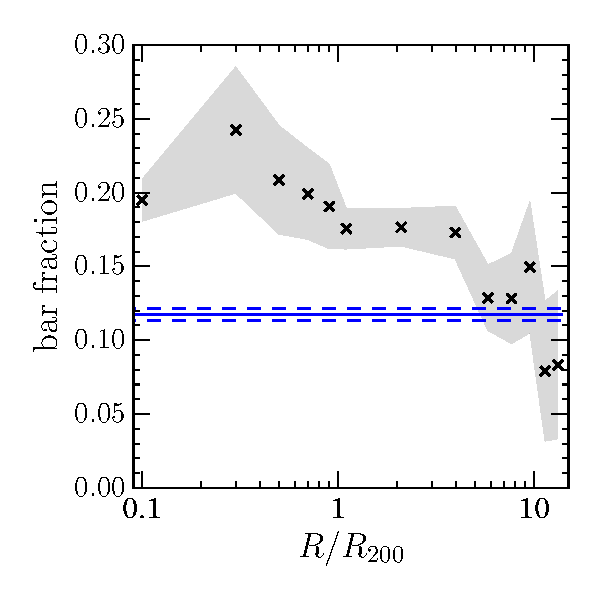
\includegraphics[width=0.46\textwidth]{environment/bar_fraction_over_disc_trend_with_log_radius_sat_matched_field_cand.pdf}}
\caption{Bar fraction (number of barred disc galaxies over number of disc galaxies) in the \textsc{gz2-group} sample binned in projected group centric radius, normalised by $R_{200}$, a proxy for the virial radius of a group. The shaded region shows $\pm1\sigma$ on the bar fraction. The bar fraction of the \textsc{gz2-sat-field} sample is also shown (blue solid line) with $\pm1\sigma$ (blue dashed line).}
\label{fig:barradius}
\end{figure}

\begin{figure}
\centering{
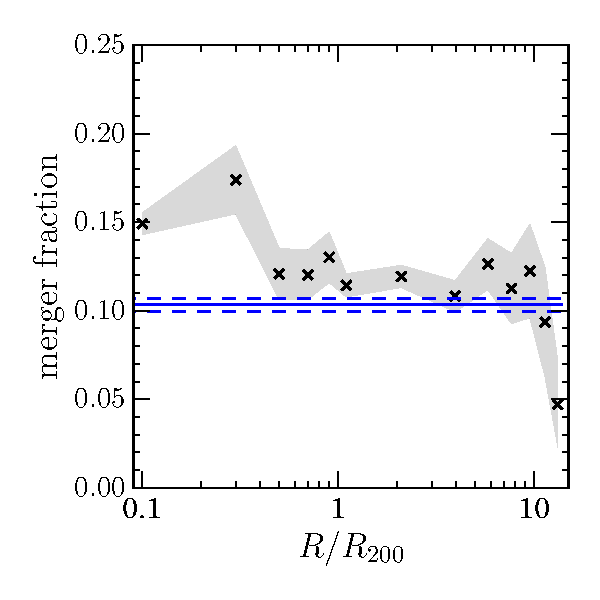
\includegraphics[width=0.46\textwidth]{environment/merger_fraction_trend_with_log_radius_compare_sat_field_cand.pdf}}
\caption{Merger fraction in the \textsc{gz2-group} sample binned in projected group centric radius, normalised by $R_{200}$, a proxy for the virial radius of a group. The shaded region shows $\pm1\sigma$ on the merger fraction. The merger fraction of the \textsc{gz2-sat-field} sample is also shown (blue solid line) with $\pm1\sigma$ (blue dashed line).}
\label{fig:mergerradius}
\end{figure}


I perform an initial sanity check on th \textsc{gz2-group} sample by recreating the morphology-density relation \citep{dressler80} in Figure \ref{fig:morphradius} which shows the mean disc and smooth vote fractions as a function of group radius. The mean disc vote fraction decreases from the mean field value (blue line) under $1$ virial radius, in agreement with previous studies on the morphology-density relation \citep{dressler80, smail97, poggianti99, postman05, Bamford09}. The extensive morphological classifications provided by GZ2 now allow for the investigation of how more detailed morphological structure is affected by the group environment.  

Figure \ref{fig:barradius} therefore  shows how the bar fraction (number of barred disc galaxies over the number of disc galaxies) increases towards the centre of the group population, significantly over the field fraction (blue solid line). Figure \ref{fig:mergerradius} shows how the merger fraction does not significantly deviate from the field fraction (blue solid line) until within a virial radius. Similarly, the left panel of Figure \ref{fig:bulgeradius} shows how those galaxies identified as having no bulge or a just noticeable bulge are less common in the inner regions of the cluster (left panel), whereas the fraction of galaxies with obvious or dominant bulges increases with decreasing projected distance from the centre of the group.

%Figure \ref{fig:sfrradius} shows how the SFR of the \textsc{gz2-group} sample does indeed decline with decreasing group centric distance, significantly below the mean SFR of the \textsc{gz2-field} sample shown by the blue dashed line. This is in agreement with the results of \cite{gomez03} who observe a similar decline in SFR with group centric radius in SDSS clusters (see for example, Figure 6 in \citealt{gomez03}). This coincides with the morphological fraction changes seen in Figures~\ref{fig:morphradius}-{\ref{fig:merger radius} in support of the conclusions of \citet{smethurst15} that quenching is morphologically dependent. 


%\begin{figure}
%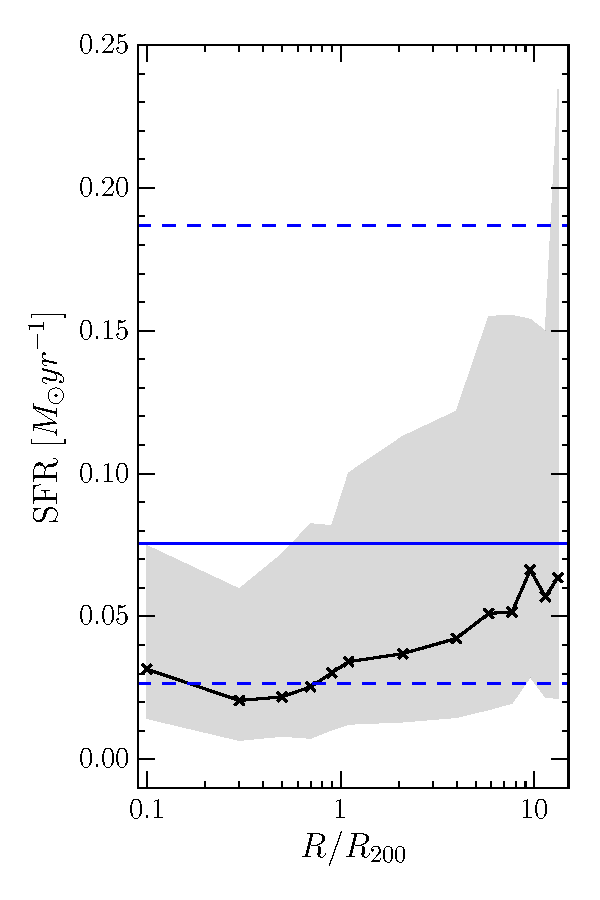
\includegraphics[width=0.46\textwidth]{environment/sfr_trend_with_log_radius_field_matched_blue_dashed_hlines_gomez_03_rv_not_r200.pdf}
%\caption{Median $H\alpha$ derived star formation rates of satellite galaxies in the \textsc{gz2-group} sample, binned in projected group centric radius, normalised by $R_{200}$, a proxy for the virial radius of a group.  The shaded region shows the SFRs encompassed by $50\%$ of the population in a given bin. The median SFR of the \textsc{gz2-sat-field} sample is shown (blue solid line) along with the 25th and 75th percentiles (blue dashed lines).}
%\label{fig:sfrradius}
%\end{figure}

\subsection{Quenching times in the group environment}

\begin{figure*}
\centering{
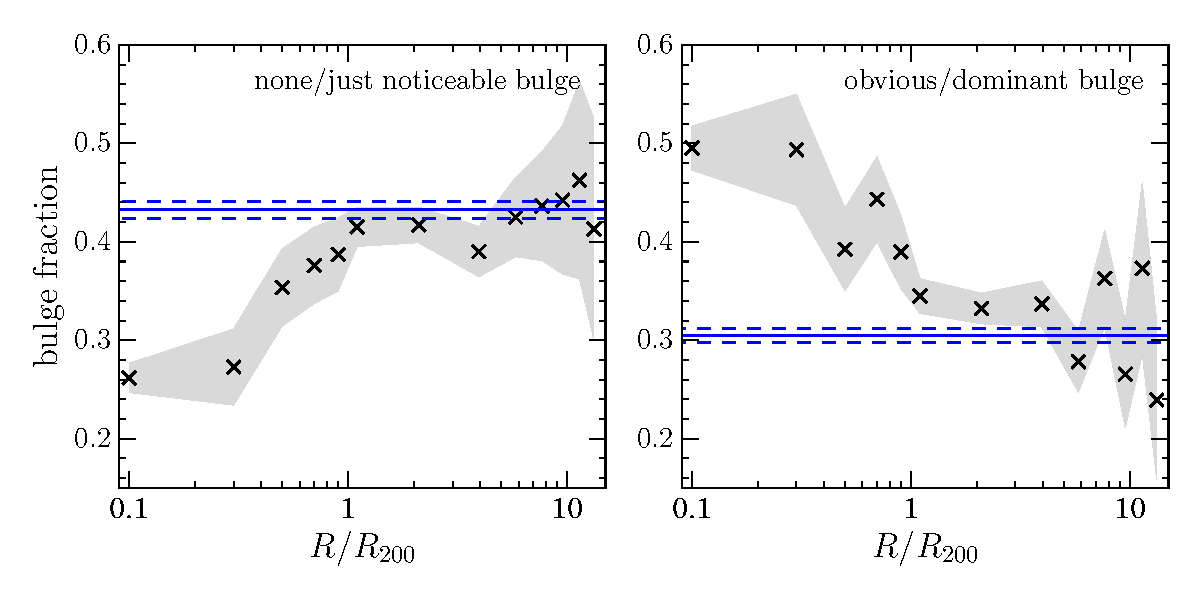
\includegraphics[width=0.85\textwidth]{environment/min_max_bulge_fraction_trend_with_log_radius_sat_field_cand.pdf}}
\caption{Fraction of galaxies with none/just noticeable bulge classifications (left) and with obvious/dominant bulge classifications (right) in the \textsc{gz2-group} sample binned in projected group centric radius, normalised by $R_{200}$, a proxy for the virial radius of a group. The shaded regions shows $\pm1\sigma$ on the bulge fractions. The bulge fractions of the \textsc{gz2-sat-field} sample are also shown (blue solid lines) with $\pm1\sigma$ (blue dashed lines).}
\label{fig:bulgeradius}
\end{figure*}

\begin{figure}
\centering{
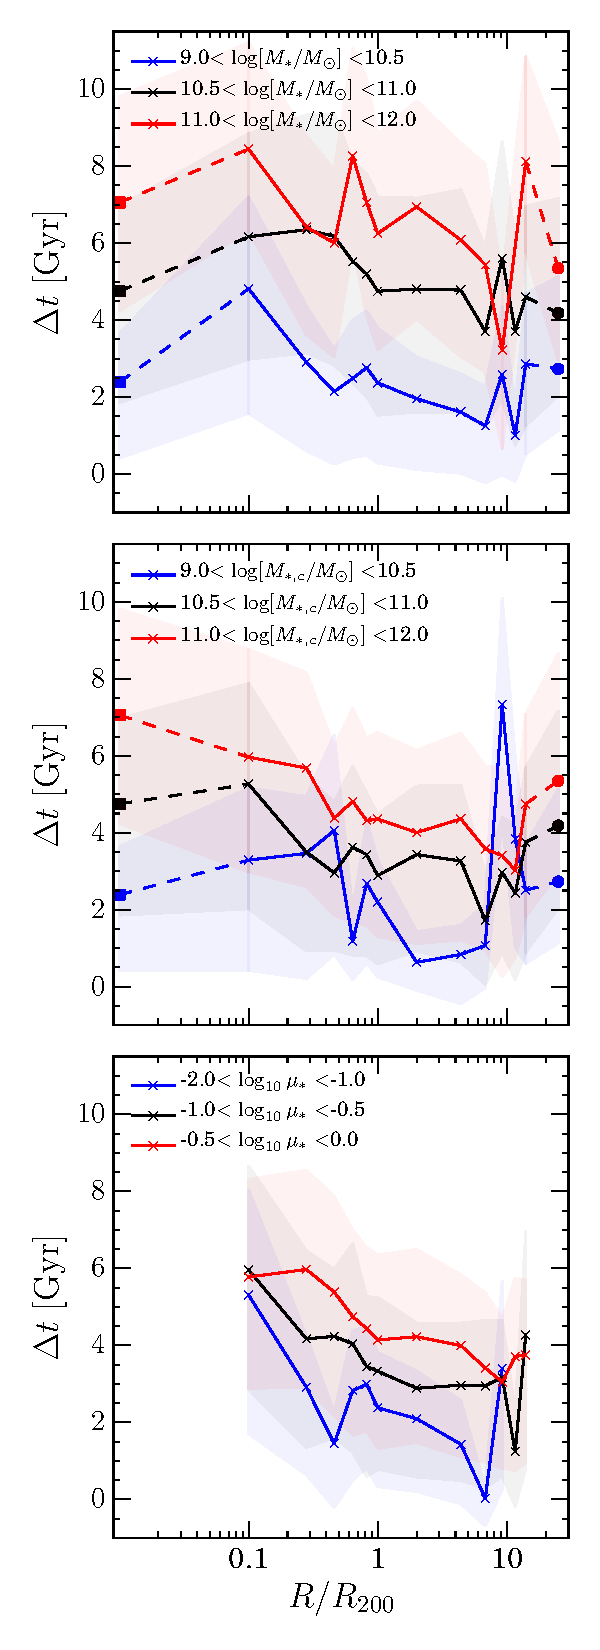
\includegraphics[height=0.8\textheight]{environment/time_since_quenching_M*_Mh_mu.pdf}
\caption{The time since quenching onset ($\Delta t = t_{obs} - t_{q}$) binned in projected group centric radius, normalised by $R_{200}$, for satellite galaxies (crosses) split into bins of stellar mass (top), stellar mass of the corresponding central galaxy (middle; a proxy for halo mass of a group) and the stellar mass ratio ($\mu_* = M_*/M_{*,c}$, bottom). The corresponding values for central galaxies (squares, plotted at $0.01 R/R_{200}$) and galaxies in the \textsc{gz2-cent-field-q} sample (circles, plotted at $25 R/R_{200}$) are shown where calculable and connected by the dashed lines to help guide the eye. The shaded regions show the $\pm1\sigma$ on $\Delta t$ in each bin of $R/R_{200}$.}
\label{fig:timesinceradius}}
\end{figure}

\begin{figure}
\centering{
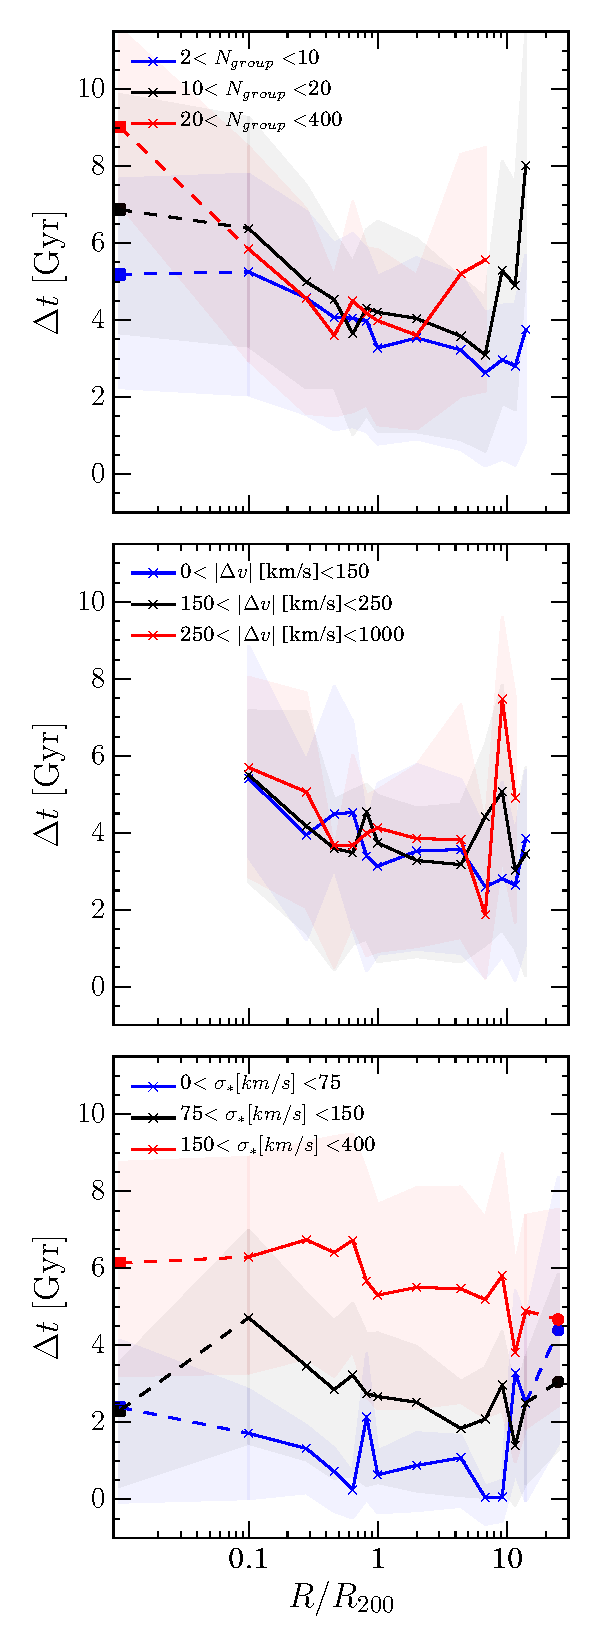
\includegraphics[height=0.8\textheight]{environment/time_since_quenching_Ngroup_delv_sigma.pdf}
\caption{The time since quenching onset ($\Delta t = t_{obs} - t_{q}$) binned in projected group centric radius, normalised by $R_{200}$, for satellite galaxies (crosses) split by the number of group members ($N_{group}$, top), absolute relative velocity of the satellite to its central galaxy ($|\Delta v|$, middle) and velocity dispersion ($\sigma_*$, bottom). The corresponding values for central galaxies (squares, plotted at $0.01 R/R_{200}$) and galaxies in the \textsc{gz2-cent-field-q} sample (circles, plotted at $25 R/R_{200}$) are shown where calculable and connected to the satellite values by the dashed lines to help guide the eye. The shaded regions show the $\pm1\sigma$ on $\Delta t$ in each bin of $R/R_{200}$.}
\label{fig:timesinceradiusvel}}
\end{figure}


With the output from \starpy~ I look at the trends in the time since quenching onset ($\Delta t = t_{obs} - t_{q}$, see Section \ref{sec:starpy}) with group radius for satellite galaxies and central galaxies in the \textsc{gz2-group} sample, compared with galaxies in the \textsc{gz2-field} sample. This is shown in Figures \ref{fig:timesinceradius} \& \ref{fig:timesinceradiusvel} with the \textsc{gz2-group} sample binned by various group properties:
\begin{itemize}

\item{Stellar mass, $M_*$: in the top panel of Figure \ref{fig:timesinceradius} galaxies in the \textsc{gz2-group} sample are split by their stellar mass and a clear trend for increasing time since quenching onset with increasing stellar mass for satellite, central and field galaxies can be seen. The central galaxies (shown by the square points at $\sim 0.01 R/R_{200}$) appear to have quenched more recently than the inner satellites (at $\sim0.1R/R_{200}$) 
of the same mass.}

\item{Halo mass: in the middle panel of Figure \ref{fig:timesinceradius} I use a proxy for halo mass by splitting the \textsc{gz2-group} sample by the stellar mass of the corresponding central galaxy of a group, $M_{c,*}$ and find a clear trend for increasing time since quenching onset with increasing stellar mass of the group central for satellite, central and field galaxies.}

\item{Mass ratio, $\mu_* = M_*/M_{*,c}$: the stellar mass ratio of the satellite to its central galaxy. In the bottom panel of Figure \ref{fig:timesinceradius} we show the time since quenching of the \textsc{gz2-group} split into bins of $\log_{10}\mu_*$. The change in $\Delta t $ with projected group centric radius occurs more steeply (particularly beyond $\sim$ a virial radius) for satellite galaxies with much smaller masses than their group central ($-2.0 < \log_{10}\mu_* < -1.0$, shown by the blue curve).}

\item{Number of group members, $N_{group}$: the top panel of Figure \ref{fig:timesinceradiusvel} shows that there is no trend with time since quenching onset with increasing $N_{group}$ for satellite galaxies. The central galaxies (shown by the square points at $\sim 0.01 R/R_{200}$) however, do show a trend for increasing time since quenching with $N_{group}$.}

\item{Relative velocity, $|\Delta v|$: in the bottom panel of Figure \ref{fig:timesinceradiusvel} I split the satellite galaxies of the \textsc{gz2-group} sample into bins of relative velocity to their central galaxies. There is no trend with time since onset of quenching with increasing relative velocity for galaxies in the group environment.}

\item{Stellar velocity dispersion, $\sigma_*$: the bottom panel of Figure \ref{fig:timesinceradiusvel} shows the time since quenching of the \textsc{gz2-group} sample split into bins of $\sigma_*$. The stellar velocity dispersion shows the largest trend in $\Delta t$ for satellite galaxies of all of the group properties studied, with galaxies with the smallest stellar velocity dispersions having quenched more recently, and vice versa. }
\end{itemize}

Across all the panels in Figures \ref{fig:timesinceradius} \& \ref{fig:timesinceradiusvel} a general trend for increasing time since quenching onset with group radius can be seen. As earlier, in Figures \ref{fig:morphradius}$-$\ref{fig:bulgeradius} significant differences from the field averages arise inside $\sim$ one virial radius. 


\section{Discussion}\label{sec:disc}

\subsection{The role of mergers in quenching in the group environment}\label{sec:rolemergerenv}

The merger classification in GZ2 has been shown to preferentially identify major mergers \citep{darg10a}; wheras, bulge formation in disc galaxies is often associated with (minor) merger driven evolutionary histories \citep{croton06, tonini16}.  Although we see evidence for an enhanced merger fraction in the inner regions of the group environment in Figure~\ref{fig:mergerradius}, the bulge fractions in Figure~\ref{fig:bulgeradius} vary much more significantly from the field value than the merger fraction. This suggests that minor mergers may be more dominant than major mergers in the group environment, particularly at $R/R_{200} > 0.5$. 

If mergers are an important evolutionary mechanism for satellite galaxies, as the morphological evidence in Figures~\ref{fig:mergerradius} \& \ref{fig:bulgeradius} suggests, we would expect to see a difference in the quenching histories of satellites residing in groups with a larger number of members. However, the top panel of Figure \ref{fig:timesinceradiusvel} shows there is no trend with time since quenching onset with increasing $N_{group}$ for the satellite galaxies. This suggests that mergers are not the dominant quenching mechanism for satellite galaxies.

For central galaxies however, this is not the case. The central galaxies (shown by the square points at $\sim 0.01 R/R_{200}$ in the top panel of Figure \ref{fig:timesinceradiusvel}), do show a trend for increasing time since quenching with increasing $N_{group}$. Therefore, we can postulate that the larger the number of group members, the more important mergers are for a central's evolutionary history. 

This idea is supported by the result shown in the top panel of Figure~\ref{fig:timesinceradius} when the \textsc{gz2-group} is split into bins of stellar mass. We can see that centrals of a given mass have quenched more recently than the inner satellites (at $\sim0.1R/R_{200}$) of a given mass. This suggests that an episode of more recent star formation may have occurred in the central galaxies but not in the inner satellites. This is once again suggestive of a merger dominated evolutionary history for central galaxies, as mergers are thought to cause an energetic burst of star formation which in turn quenches the remnant galaxy \citep{hopkins05, treister12, pontzen16}. If the central galaxies have quenched more recently than the inner satellites this could be a more recent burst of star formation caused by a merger under this regime. 


\subsection{The role of mass quenching in the group environment}\label{sec:rolemassenv}

The role of mass quenching in the group environment is apparent in the top panel of Figure~\ref{fig:timesinceradius} and the bottom panel of Figure~\ref{fig:timesinceradiusvel} where the \textsc{gz2-group} satellites are binned by stellar mass and central velocity dispersions respectively. We see a trend for increasing time since quenching with increasing stellar mass and velocity dispersion for centrals, satellites and field galaxies. This is suggestive of mass quenching occurring across the entire galaxy population irrespective of environmental density, supporting the work of \citet{Peng10, gabor10, peng12} and \citet{darvish16}.

\subsection{The role of morphological quenching in the group environment}\label{sec:rolemorphenv}

The results in Figure \ref{fig:barradius}, showing the increasing bar fraction towards the central group regions which is consistent with results that show that bars themselves may be the cause of morphological quenching through the funnelling of gas toward the central regions of galaxies \citep{athanassoula92b, sheth05,masters10c}. However we must consider whether the environment itself may play a role in triggering the disk instabilities which can produce a morphological bar. Indeed harassment and tidal interactions have been shown to both promote and inhibit bar formation dependent on the stellar mass \citep{noguchi88, moore96, skibba12}.  In this case, morphological quenching would be occurring but indirectly due to environmental quenching. 

\subsection{The role of the environment in quenching}\label{sec:roleenv}

Across all panels of Figures ~\ref{fig:timesinceradius}-\ref{fig:timesinceradiusvel} a trend for increasing time since quenching onset with decreasing projected group centric radius is present. This suggests that the environment does directly cause quenching throughout the infall time of a galaxy in a group. Those galaxies closer in, fell into the group earlier and as they did so they started to quench, giving rise to a larger inferred $\Delta t$.

The results in Figure \ref{fig:timesinceradius} suggest more massive halos therefore have a greater impact on the star formation histories of their satellites than less massive halos. The stellar mass of the central galaxy is used as a proxy for halo mass which is correlated with both (i) the gravitational potential of the group \citep{ref} and (ii) the temperature of the IGM \citep{ref}.

It is thought that higher mass halos have hotter inter galactic medium (IGM) temperatures \citep{ref} which can then have a greater impact impact on a galaxy through RPS of cold gas \citep{ref}. If RPS is indeed a dominant environmental quenching mechanism we should see a trend in $\Delta t$ with the speed of a satellite galaxy relative to the group central.  However in the middle panel of Figure \ref{fig:timesinceradiusvel} we see that this is not the case. 

This suggests that any environmental quenching mechanism responsible for the trends seen Figures~\ref{fig:timesinceradius} \& \ref{fig:timesinceradiusvel} are not correlated with satellite velocity. This therefore rules out RPS as the dominant environmental quenching mechanism, in support of the conclusions of simulations by\citet{emerick16, fillingham16} and observations by \citet{mcgee14}. 

The dominant environmental quenching mechanism in the group environment must therefore be correlated with the group potential. This suggests that satellite galaxies may be most affected by gravitationally driven environmental effects, such as harassment and galaxy-galaxy interactions or by thermal evaporation of the galaxy halo due to the hot IGM. 


\section{Conclusions}\label{sec:conc}

Mergers, mass quenching morphology quenching and environmental quenching are all prevalent in galaxy groups. The environment does play a role in quenching galaxies through a mechanism proportional to the halo mass of the group but not proportional to the relative speed of the satellite galaxy to its central galaxy. This suggests that ram pressure stripping is not the dominant environmental quenching mechanism. All of these mechanisms discussed coalesce to give rise to the distributions in galaxy properties we see across the Universe through their constant interplay across cosmic time. 

